Für die in diesem Bericht durchgeführten Messungen wurden zwei Versuchsaufbauten verwendet. Zum einen der Aufbau zur direkten Beobachtung und zum anderen der Aufbau nach der frauenhofer'schen Beobachtungsart. Die zwei Aufbauten werden hier etwas detalierter aufgeführt.

\subsection{Direktes Beobachten des Fernfelds} \label{sec:direkt}
%%%%%%%%%%%%%%%%%%%%%%%%%%%%%%%%%%%%%%%%%%%%%%%%%%%%%%%%%%%%%%%%%%%%%%%%%%%%%%%
% pictures
\begin{figure}[htb]
\center
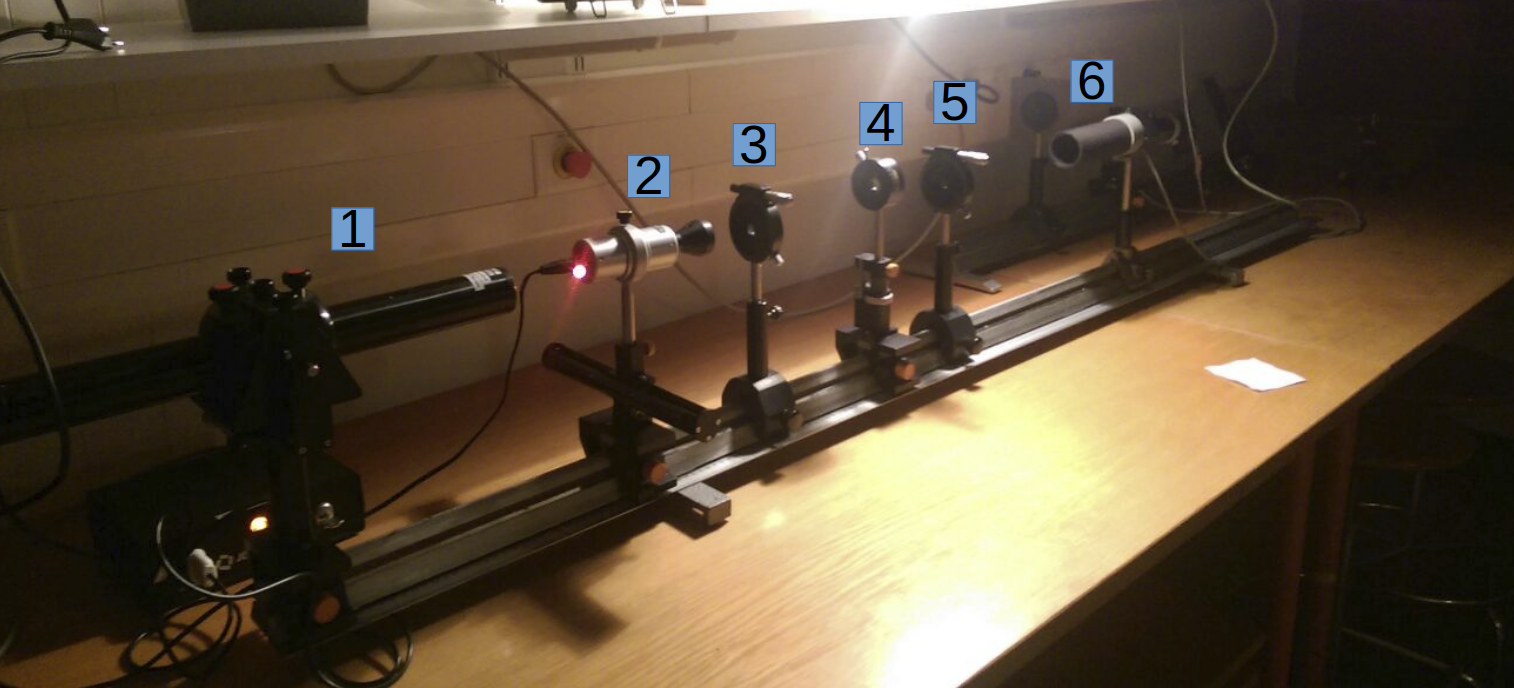
\includegraphics[width=\textwidth]{graphics/versuchsaufbau.png}
\caption{Versuchsaufbau Direktes Beobachten} % picture caption
\label{fig:direkt}
\end{figure}
%
%(Abb. \ref{fig:image1})
%%%%%%%%%%%%%%%%%%%%%%%%%%%%%%%%%%%%%%%%%%%%%%%%%%%%%%%%%%%%%%%%%%%%%%%%%%%%%%%

\begin{tabbing}
\hspace{20mm}			\= 	\\
1)	\>	He-Ne-Laser Rot $\lambda$ = 632.8nm 5mW	\\
2)	\>	NdYAG Laser Grün $\lambda$ = 532nm 5mW	\\
3)	\>	Polarisator Glan-Thompson Prisma	\\
4)	\>	$\lambda / 2$ Wellenplatte für 632.8nm	\\
5)	\>	Analysator Glan-Thompson Prisma	\\
6)	\>	J16 Digital Photometer			\\

\end{tabbing}

\textbf{Messvorgang}\\
\\
Das zu Messende Objekt wird in den Objekthalter eingeführt. Die Distanz des Objekthalters zur Mattscheibe wird so eingestellt, dass die Maximas auf dem Schirm gut ersichtlich sind. Es sollen links und rechts von der Mitte 4 maximas ausgemessen werden können. Danach wir die Distanz des Objekthalters zur Mattscheibe mit einem Doppelmeter ausgemessen. Die Distanz der jeweiligen Maximas, auf der Mattscheibe, wird mit der dafür vorgesehenen Vorrichtung ausgemessen.
\clearpage
